%************************************************
\chapter{Introduction}
\label{chapter:introduction}
%************************************************

In this dissertation, I present the substrate for accountable layered systems.
I have focused on building this substrate for doing reflective thinking on a large scale in learning systems.  \cite{singh:2005}'s example of reflective architectures is a good precedent.
I will go over the contributions of this thesis.

\begin{itemize}
\item The Substrate
\item The Simulation
\item The Model
\end{itemize}
  
\section{The Substrate Contribution}

My primary thesis contribution is the substrate.  The substrate is a
system for developing large software applications, practical systems.
This enables parallel and concurrent process control.  When you have
hundreds of parallel processes, you can pause these processes.  When
they get bugs, you can look at them; they are paused state machines.
There are intricate thread control operations for these processes.
When they sleep, they are removed from the scheduler, focusing
computational resources.  Thousands of sleeping processes can
efficiently be "triggered" awake.  The primary point of the system is
that when running many different problem solvers at the same time, it
becomes convenient to trace the interactions between those problem
solvers.  Thus, all of the memory in this substrate allows tracing all
memory allocation and mutation.  It is a frame based system.  Many AI
systems are implemented in an object-oriented or frame-based
representation.  This allows for all of the commonly associated
programming methodologies to exist, i.e.  object types and
inheritance, etc.  The substrate includes a high-level lisp-like
programming language, so the compiler can be redefined by the running
program.  There are layered cognitive architecture structural
primitives included in the language.  If you want to build a ``layer''
which contains ``agencies'' which contain ``resources'' which exist as
``minds'' which control ``physical worlds'', all of those primitives
already exist in this substrate.  This substrate serves as an
extensible platform for continuing research on this implementation of
reflective thinking.  You can download this open-source software and
begin doing this kind of research.

\section{The Simulation Contribution}

My second thesis contribution is a mathematical description of a
simulation that gives an answer to the following questions: How do we
do credit assignment for learning?  When you have all of these
processes interacting, solving a problem, which may be a complicated
parallel system in itself, how do we trace the credit for our
decisions that we have made in performing actions?  What knowledge was
that decision based on?  How do we trace that backwards in time in an
efficient way?  How do algorithms currently assign credit backwards in
time and how does this model relate to these methods?  By describing
the mathematical simulation, I will evaluate how this model's ability
to learn not only at the ground level but also at the knowledge
manipulation level improves over just ground learning performance.

I will evaluate this simulation as a potential path around the
combinatorial search explosion problem.  There is a certain ``curse of
dimensionality'', so if you approach a large domain with many
dimensions, you try to generalize the state space in abstract terms,
such as logical relationships.  Large systems that have logical
relationships, hundreds of thousands, millions of relationships, fail
because there is this explosion of combinatorial search.  I describe
the simulation as a path around the search problem, anything that
involves search.  The details of the simulation model are the basis of
the computational substrate.

\section{The Modelling Contribution}

My third thesis contribution is a reflective model of mind that gives
a description of how to think about learning to control.  There are
many models for learning to control.  I describe a model that has not
been explored by many of the current machine learning disciplines.
This model of mind is the basis of the mathematical simulation.

\section{Document Overview}

The focus of the dissertation will be on a description of the learning
to control problem.  I describe control in terms of layers of
reflective credit assignment because I think this simplifies
understanding the learning to control problem.  I will focus on how
credit assignment is done at the level of the planning activities.  I
will then describe multiple experimental implementations of this
reflective model of mind, simulations of controlling two different
physical domains of varying complexity.

\section{Programming}

An example problem domain called the block building domain is shown in
Figure~\ref{figure:example_problem_domain}.  In this case, we have two
blocks.  They have relationships with the objects in the room, such as
the table.  The goal state is the stack of {\tt Block-2} on top of
{\tt Block-1}.  The goal is to get the physical world to exist in this
sort of configuration.
\begin{figure}
\center
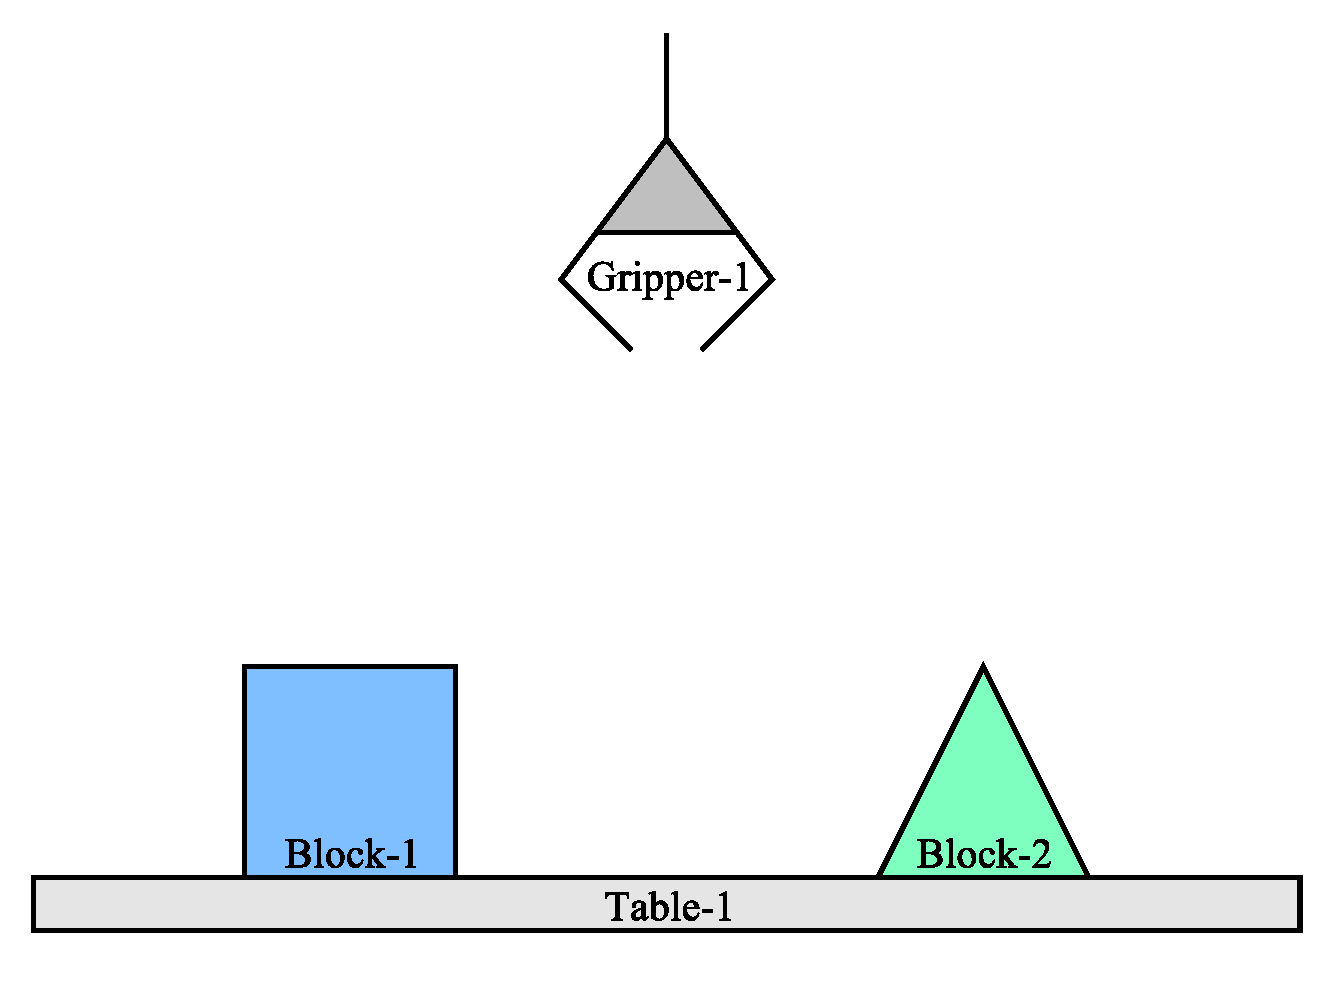
\includegraphics[width=10cm]{gfx/blocks_world_example-1}
\caption{An example problem domain.}
\label{figure:example_problem_domain}
\end{figure}

Figure~\ref{figure:example_program} shows an example of a program that
a programmer might write to move this gripper around in this block
building domain.  In this program, the gripper has very simple
symbolic commands: {\tt move-right}, {\tt grab}, {\tt move-left}, {\tt
  drop}.  One can imagine that this program might mean to pick up the
green block and put it on the blue block.  This is what programming
is, very abstractly.
\begin{figure}
\center
\begin{tabular}{l}
\\
  {\tt ~~[defunk example-program []}~~ \\
  {\tt ~~~~[move-right]} ~~\\
  {\tt ~~~~[grab]} ~~\\
  {\tt ~~~~[move-left]} ~~\\
  {\tt ~~~~[drop]]} ~~\\
\\
\end{tabular}
\caption{An example program.}
\label{figure:example_program}
\end{figure}

\section{State Space Planning}

State space planning can be thought of as automatic programming.
Planning is when the computer writes the program itself.  In a simple
planning as search algorithm, there is an initial state with a number
of possible actions that may lead away from this state.  We can move
left; we can stop; we can move right.  We can imagine what the
possible future states would be after each action.  In an imagined
future state, the gripper may be in a different position.  We can
continue this process.  This is the explosion of the combinatorial
search.

every single step if it has the same number of actions becomes this exponential search problem, which really slows the algorithm down.
so, this process goes on as much as we can computationally afford, and then you end up moving closer to making your, finding your goal state in this large space of all possible alternatives.
what we can do over this search process, is develop heuristics.
so, basically, we have weightings, so for every action that we can take from each state, we basically have a very myopic kind of not necessarily myopic but an algorithm that will spit out a number that ranks all of these different search paths.
so, if we think heuristically that moving red blocks before moving green blocks is a good idea, we don't exactly have a proof for it, but we can program that in as a heuristic, then the search path will more likely going along those paths.
and it ends up reducing the branching of the search tree.
that's what we really want to do when we attack the search problem is if we reduce the branching factor, we basically reduce the search problem.
so, here's the path that we might take, given that we've only gone along the preferred heuristic paths.
the green one would be our solution.
so, that's a plan.
that's part of the problem.
how do we represent actions?
so, each of these specific actions needs to be represented in a way so that we can use it to simulate the physical world.
so, there are examples, STRIPs use a formulation called "trans-frames" which is basically, given a representation of the state of the world, a transframe is a list of additions and a list of removals from the world.
and so, if you have this basic relational domain, block-1 is on block-2.
one transframe might say, remove block-1 from on block-2 from our knowledge of the world, and add block-2 on top of table, something like that, changing the world through transframes.
the problem that STRIPs has in imagining the effects of actions on the world is that this requires you, basically, it doesn't consider the current state of the world.
so, basically, given an action it will change the world in this given way.
you add these things.
you remove these things.
so, if we want to make this simulation dependent on the current state of the world, we have to somehow make a decision in terms of, what is the current state of the world, and what should the transframe be given this action.
there are many ways to solve that problem.
one simple one is to enumerate all possible actions and state spaces and say there's a different transframe for each one of those.
that's an inefficient way of doing that.

so, in the blocks world, we can imagine transframes that are dependent on the current state of the world by,
let's say, if the block is glued down to the table, and we can see that.
then we can execute the grab action from when the gripper is above the block, and the block won't be removed from the table.
so, that's a different transframe than for if the block was not glued to the table, then we could imagine that then the block would then be in the gripper's grip.
so, two different transframes for the same action.
so, actions are dependent on the physical world in blocks world.
in the real world, you can imagine eating a sandwich, and if it's not your sandwich it would have completely different effects than if it was your sandwich.
obviously, actions have a depdence on the physical world.

so, let me go through briefly, once we have predicted the effects of our actions.
we can basically predict, we have used a decision based on the physical world to predict which transframe is appropriate for simulating this action.
so, what that allows us to do is to have causal dependencies between the knowledge used for generating the decision, and the actual future state of the world that has been derived from that.
so, the current imaginary state of the world through the decision knowledge to the future state of the world has these causal relationships.
so, along time here, what i've drawn is basically as the algorithm is simulating forward knowledge is dependent on certain things in the past but not necessarily in a temporal order it really depends on when the decision was made, what knowledge the decision was based on, and what knowledge that ended up creating.
you can imagine something being learned far in the past, and the decision that uses that learning process may be done far in the future.

the problem becomes when we get a bug in the system.
so, imagine that this is a plan that has been created over time.
we've imagined simulating the world and we've developed this plan.
when we're executing this plan, which has these sorts of causal relationships back in time, we hit a bug in the execution in the plan.
that's what this red dot here symbolizes.
so, basically, what traditional temporal learning algorithms will do, they go back to the previous time step or the previous action, and they say, this is what's responsible for this, we should relearn the preconditions and postconditions for this action, we should recategorize the world for this action, we should focus on this action, and maybe the one before it, and we can kind of continue this process backwards in time.
reinforcement learning has a temporal difference algorithm that does this.
it is a pretty standard reinforcement learning algorithm.
this is pretty standard.
you can make hierarchies of actions.
you can make longer spans in time.
the basic theory is that you back to the previous timestep, what action was happening?, and then you can go to the timestep before that action.
this is a different approach.
this doesn't go back in time to the previous action.
this goes back causally through the provenance of the knowledge.
so, in this case we can follow this blue path, and since we know that this faulty piece of knowledge came from that way back piece in time, we can actually go back and we specifically focus on that decision that was possibly even in a planning process.

so, i'm talking about reflection.
reflection is an overused word in this field.
it's kind of diffisult to read the literature
pattie maes, not to just throw out her name because she works here, but she actually has a really good paper that describes about 30 different types of definitions for reflection that are grounded in the computer science literature.
i'm going to go through three of them.
one of them she doesn't talk about because its not computational reflection, and this is actually the one that i'm focusing on in this phd.
reflection is, basically, in a laymans psychological term, is what i'm trying to model here.
so, reflection is the act of perceiving acting and otherwise controlling your basic deliberative thought process.
so, if you have a thought process that is going through this planning process, weighing decisions, making plans, and trying to accomplishg goals, that's what i'm calling a deliberative thought process.
so, the process that is optimizing that, for example, learning heuristics for the search, would be a reflective process.
so, what reacts to the bugs and relearns the planning processes and does the sort of causal tracing.
that's the high level kind of meta-congitive definition of reflection that i'm trying to focus on.
there's two other places where reflection is used.
one of which i'm going to continue to call reflection, but i'll usually note when it is this type.
computational reflection is simply there's a lot of different types of computational reflection and i would point you to pattie maes work on that to understand it more.
there's a procedural reflection, which involves a meta-circular evaluator which i haven't built, but i'm basically doing something similar in that I have an interpretter that will give you events as it interprets the program.
its a bytecode interpretter and it is a compiled language, but i basically can do this tracing of a process as it runs creating events relatively efficiently.
i'm referring to that as computational reflection because that's not a very high level idea.
that's basically just as a process runs, you can see the events that are happening.  low level events, high level events, whatever.
and those are all pretty much the foundation for the rest of the whole system, which we can then build causal tracing out of.
which is a specific type of tracing that has to do with making decisions that are learned from the environment
and this involves, i'll get into this, but it involves making hypotheses keeping track of how those hypotheses are supporting each of those pieces of knowledge and if that knowledge is then used for other decisions.
so, i've gone into this a little bit.
i don't need to go into this too much.
the different between temporal learning and causal learning.
basically, if you go back to previous time steps just because they happened before that's called temporal learning.
there are a lot of those types of algorithms that currently exist.
the causal learning hasn't been done too much, and so this would help a lot of the traditional types of learning systesm.
right, and i've gone through the example where if the block was glued to the table and you did fail, you could go back to the decision that was created, so basically, debugging the decision that made that plan.
so planning systems do need this information.
planning systems don't currently keep track of this information.
so, provenance and causal learning.
so, every decision that is supported by a hypothesis, well, basically, every decision is supported by a hypothesis, so if we were to learn a category from the environment that would predict the effects of our actions, then the knowledge that is generated from that contains these references to the hypotheses that were used to create that decision.
and so, if we do find a bug in the future, we can focus on those specific actions.
and each of these will have specific types of debugging responses.
depending on which actions they are referring to.

i'm talking a lot about hypotheses.
i'm talking a lot about decisions.
let me just go through a simple example of what a decision is because this becomes very confusing very quickly if we don't ground that idea out.
this dog looks hungry should i feed him?
he may bite me.
this is a basic decision, so let's say we have two options
how do we think about modelling these two options.
we're in a current state
it could possibly lead to two other states
the question is: what action should we take?
there is a lot of complicated processing that could into making this decision, but if we just want to talk about the basic development of what a hypothesis is and how do we develop the provenance of data based on that.
that's what i'm building this up to.
we have to choose of all of the knowledge we have, maybe from the current state, maybe from the past, which should this decision be based on?
that's a very complicated problem.
generally these algorithms are focused on a dataset, so they're not required to learn those types of relationships.
how should i weigh my relative goals into this decision?
certain algorithms will have a clear ranking of goals, like a reinforcement learning algorithm will have basically, any time you get into an important state, it will give you an exact number, this state was worth this much.
this state was worth ten.
this state was worth negative ten.
the system that i'm talking about is a little more general than that.
it uses multiple goals.
they can have partial orderings.
but you have to consider, some of the may not even be directly related, so you may have to, part of this decision process could be coming up with that partial order.
i'd like to dog to not be hungry.
i also don't want to be bitten.
you're defining the states of the world that you're going to pay attention to.
what might be the results of this?
what might be the relationships?
what are the relationships now that might help us to make this decision?
for example, the properties of the dog that we might be paying attention to.
let's say, there is a hunger for the dog.
he looks hungry or he looks full.
these are all things that we're perceiving to make this decision.
the dog has a color, a breed, it could be barking or not, its going to tell us whether or not the dog is going to bite us basically.
how do we develop a hypothesis?
we may have multiple sets of training data.
this may be our first example.
we want to take the current situation and we want to make a prediction.
what kind of hypotheses could we use?
what does a hypothesis even look like?
if we feed the dog, there are a bunch of things that might happen.
he could fall asleep.
he could continue to be hungry.
here's a set of examples.
imagine that we're feeding these examples into the algorithm 1 through 4 on the lefthand side there.
there are a number of properties that we could then categorize into, for each of these numbered examples we could predict the category on the right.
we're trying to predict whether or not our hand was bitten given the features on the dog.
it's basically a function approximation algorithm that we're trying to develop as a hypothesis for this state space.

minsky: mark twain had advice about buying a stock.
if it goes up sell it.
if it goes down don't but it.

bo: i think there's a loop in that causal chain.
i've tried to avoid those.

what's the point?
why are we talking about this?
goals!
because we have goals.
there are good parts of the world
there are bad parts of the world
we want to know how to get to the good parts and avoid the bad parts
we have avoidances
we have goals
we have states of the world
these might be partial states of the world that we want to pursue or avoid
deciding on an action depends on weighing these considerations
what is the state of the world going to be?
which parts is it going to contain?
to make this categorization, here's an example.
very simple algorithm is relatively efficient for doing what it does for getting conjunctions of features as hypotheses for what might predict a category.
for example, this line here, the first two question marks with "pitbull yes" means "if the statement contains pitbull and it contains that the pitbull is barking then it is categorized as this type of category."
you can imagine the more general hypothesis is that every dog is going to bite me
that's all question marks, any of these features match.
the most specific hypothesis is that none of these features could possibly match
no matter what feature you tell me its always going to not bite me
it is a perfectly safe dog.
these are one example and then two ends of the range of this hypothesis space.
so, hypothesis h of x is a function that takes state x and predicts whether or not it is an instance of a category.
what are all of the possible hypotheses that we could learn?
this is called the inductive bias of the algorithm.
this is the assumption that we come to the state space with a certain language that we're going to describe our hypothesis within.
in general this could be a very complicated language.
in this case its very simple.
it is just a conjunction of features.
it helps us to think of these features.
i'm just going to go over these quickly because this is not fundamental to the theory, but this is just showing that we can efficiently implement a search over the entire hypothesis space.
we can use a general to specific concept ordering.
if we consider one concept always predicts that this is a positive category whenever this other concept predicts that its a positive category, then we can say that the hypothesis that predicts it more often is more general than the hypothesis that predicts it less often.
h 0f j would be the hypothesis that predicts it more often, h of k would be the less often predictor, so there an implication reelationship between every positive instance of h of k to h of j.

making decisions given hypotheses.
we have collections of these hypotheses that we can efficiently keep track of.
given training input into this algorithm.
this is called the version space learning algorithm, which i'm not going into the details of because it isn't important.
we have hypotheses represented.
we have collections of every single hypothesis that matches the given training input
we can efficiently keep track of that
given a new training instance we can run it through this decision machine to predict what the output is going to be
when all of our hypotheses agree, we know that we can be confident in our prediction
when the hypotheses disagree, this is given the assumptions of the version space learning algorithm, which means that the hypothesis that we're looking for is actually in the hypothesis space that we've chosen and things like that.
if all of the hypotheses agree, then we know that this is the right answer.
the hypothesis is in that space and it would also agree.
when the hypotheses disagree it becomes a lot more interesting.
so, how do we make decisions?
it could go one of two possible ways depending on if our hypothesis is in one set or the other, but we still act
we make some kind of assumption there.
there are probabilistic formulations of this for decision theory that says "all of my hypotheses are equally likely"
you need a prior on your hypothesis space that gives some kind of weighting on these things so that you can make a decision
there are 10 hypotheses that say yes there are 5 that say no, given that they're all equally probable, i'm going to take the one that says yes.
you can make those decisions.
you can apply those assumptions to this algorithm.

in any case, you do have to make a decision, if you do make the decision which is useful, then you can keep track of that decision's knowledge.
yes, i'm going to imagine this state of the world.
you can associate with that knowledge the hypotheses used to generate it.
you can even imagine going both ways.
if you consider that both of these are possible outcomes, you can imagine both possible states given the hypotheses that derive them.
we understand decision making.
the definition of the hypothesis is relatively clear.
the tracing the provenance of data is relatively clear.

the causal tracing of processes.
this is the low level computer science graphic of how you would trace a process.
we have low level commands or events that we are told to execute.
this is a normal AI program that is just running without reflection.
we can imagine a loop being hardcoded into this algorithm, a sequence of events that has pointers back to loop.
there's the process sitting there in memory.
we can run this process.
we can take a virtual machine.
this is loading the process into the execution register of the machine.
it starts running.
that's all the execution register knows how to do.
it just interprets and starts running.
this is what a normal AI system will do.
you load the program into the processor and it executes the program.
what we've added to this is the creation of semantic events.
when something important happens in the process below, we create a sequence of semantic events.
things that might be important to keep track of.
this function is just beginning its an important function so maybe you should know about that.
that function has exited successfully.
there were not bugs in it or i wouldn't have gotten here.
keeping track of all of these kinds of events can give us knowledge to reflect over the process.
its a basic low level computer science, computational reflection.
i'm going to distinguish that from the psychological word of reflection which i'm going to use to refer to controlling the deliberative process.
we keep track of these semantic events, which then we can recognize.
oh this pattern looks like this function is entering.
this function looks like this function is executing.
we can then have responses that happen in parallel to the basic running process.
there is an efficiency thing that we can talk about here.
the tracing of the events require a constant time slowdown.
algorithmically, that isn't a slowdown, theoretically, its big O notation.
this algorithm is running the same speed and now we've added computational reflection to it.

gjs: what is this diagram showing?
i'm confused.

bo: there is a list of.  we can think of these as low level instructions to a machine, like bytecode operations.

gjs: yes.

bo: these bytecodes have a jump from the C to the W there.

gjs: right.

bo: this virtual machine is like a thread.

gjs: yes.

bo: you can load this program in to have the thread start running it.
then on the top we can keep track of a trace of semantic events.

gjs: i'm confused about these top things that look like a sliding R on a little device I could carry around.

bo: this is meant to be a physical analogy.
it's kind of like chemistry with the dna.

gjs: i'm trying to figure out what its an analogy to.
what are you trying to actually

bo: right.  let me describe the analogy and then i'll describe how its implemented.
the analogy is that we have dna.
we have transcriptase running along the rna
and its creating amino acids that end up folding into proteins.
what this end up doing is it reads along this chain and its creating this string, which is basically, these are the amino acid codons that i want to be attaching to me.

gjs: is the string the one in the purple?

bo: the string is the one in the purple.

gjs: yes, okay.

bo: these are the codons that i want to attach.
these basically represent the amino acid binding.

gjs: these things on top are patterns.
is that what they are?

bo: these are patterns.

gjs: they match something?

bo: right.

gjs: ah.  thank you.

bo: they're meant to be floating around and then they float down and bind to the string.

gjs: okay.

bo: this is the physical analogy.
how that's implemented is you have a stream with multiple listeners each one recognizing a pattern.

gjs: fine.

bo: i use the physical analogy because there's parallel processing.
you can imagine the basic transcriptase running along the molecule without worrying about slowing down the other molecules around it in their physical simulation.
we can have responses that are other processes that immediately begin running concurrently.















\section{leftovers...}

My thesis is SALS, a computational simulation of a model of learning
in multiple reflective layers.
\autoref{figure:example_problem_domain} shows an example block
stacking problem domain.  I begin my explanation with a description of
the example problem domain:
\begin{quote}
There is a table.  Some blocks are on the table.  The blocks are of
different shapes and colors.  One of the blocks is a green triangle.
Another block is a blue square.  A gripper can move around, picking up
and putting down blocks.  Plans are made for the gripper to arrange
the blocks into different configurations.  Plans are followed that
sometimes result in a failure.
\end{quote}

%\begin{figure}
%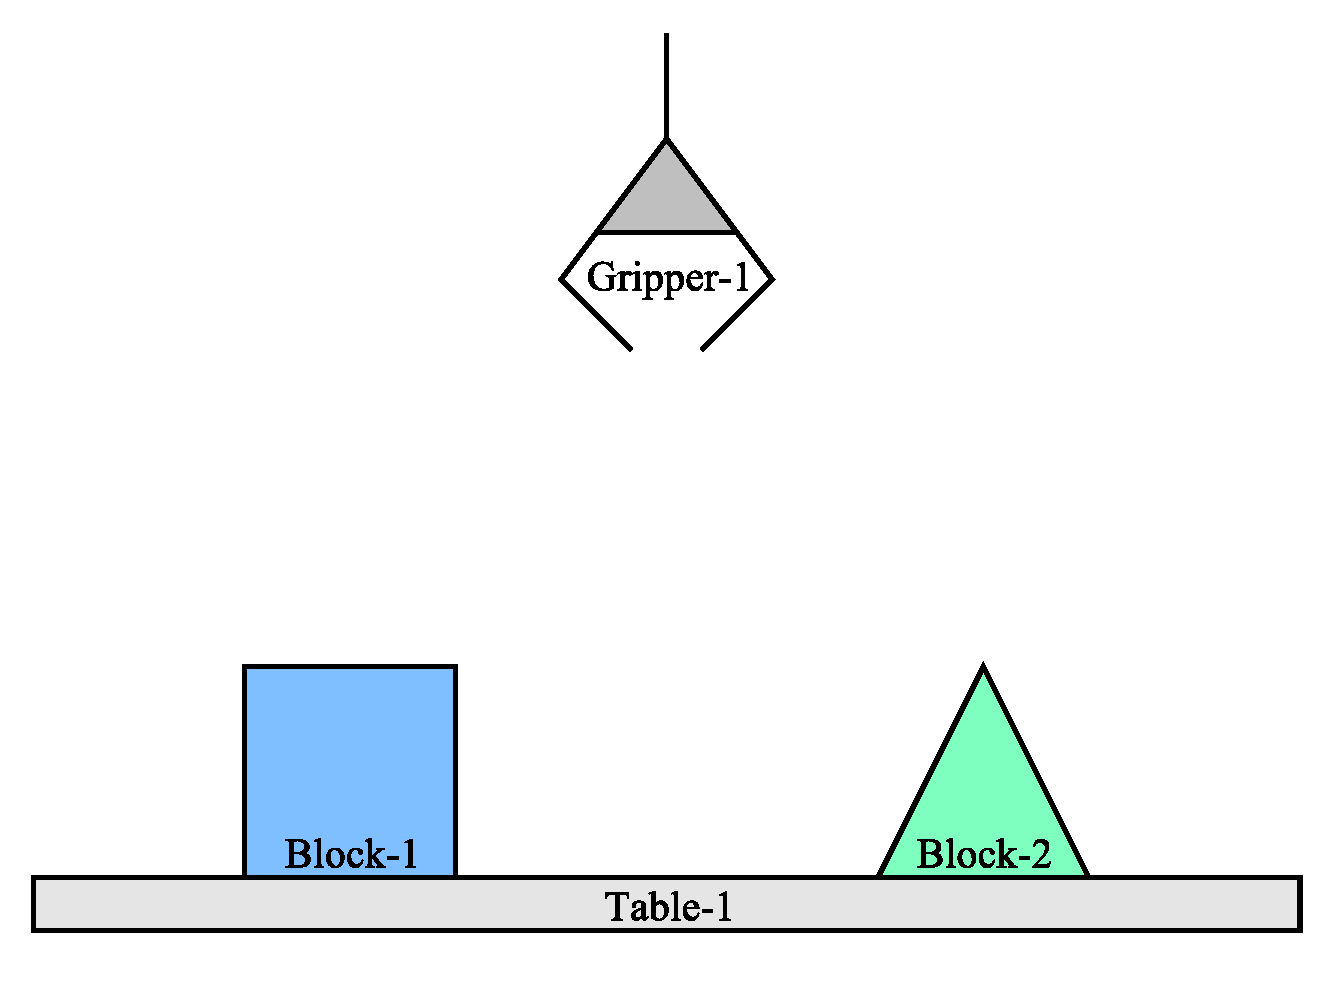
\includegraphics[width=10cm]{gfx/blocks_world_example-1}
%\caption{An example problem domain.}
%\label{figure:example_problem_domain}
%\end{figure}

\section{Example}

For example, putting the square on top of the triangle fails to stack
the two blocks because the square falls off of the triangle.  A single
failure is a learning opportunity.  A better model of the world can be
learned through each failure.

\begin{figure}
\begin{tabular}{p{5cm}p{5cm}}
1.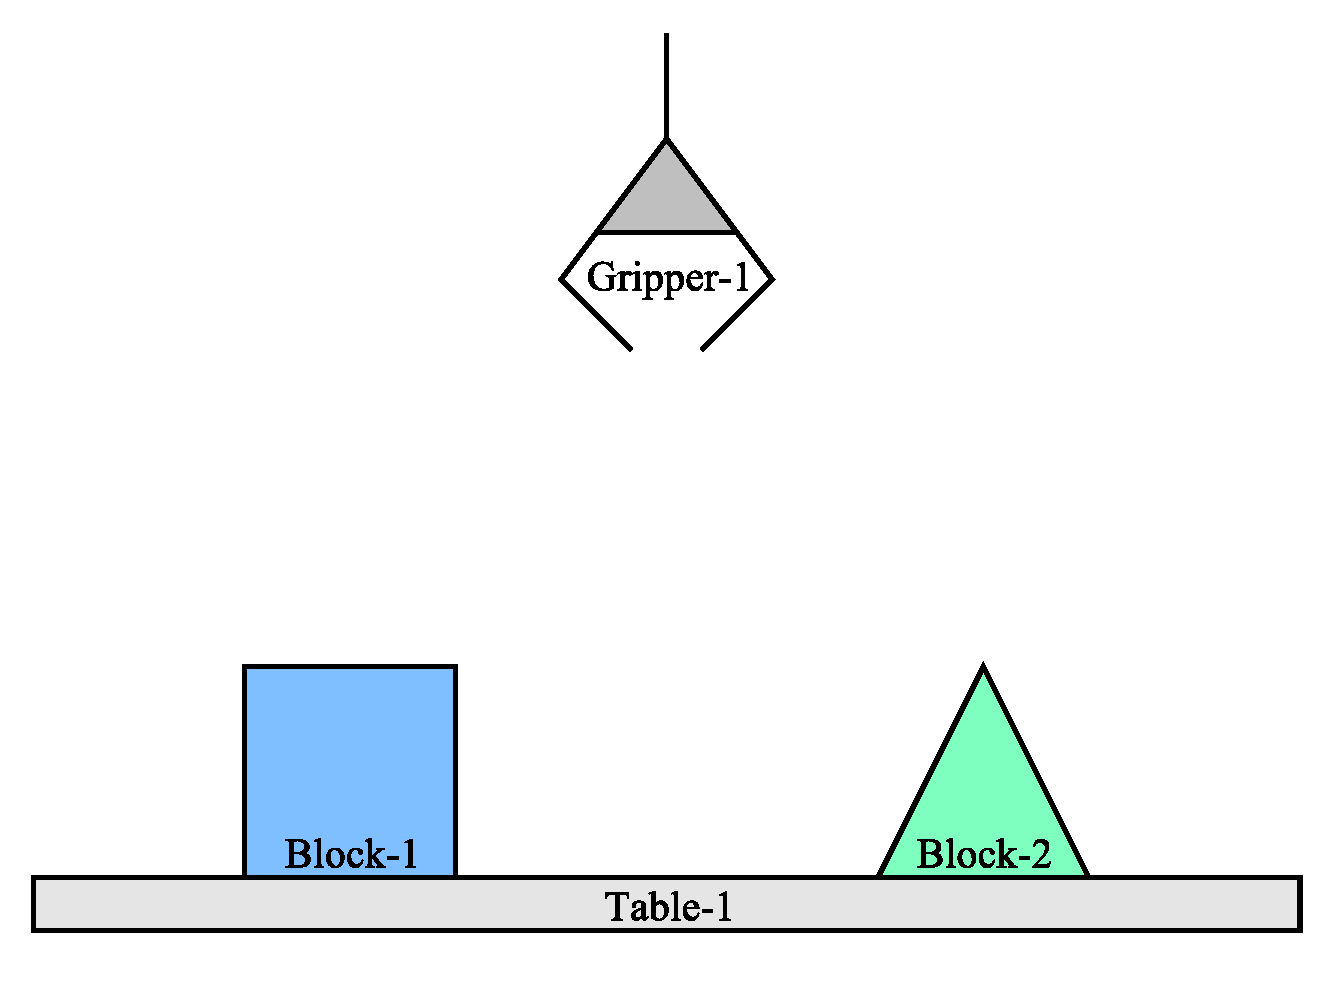
\includegraphics[width=4.5cm]{gfx/blocks_world_example-1} & 2.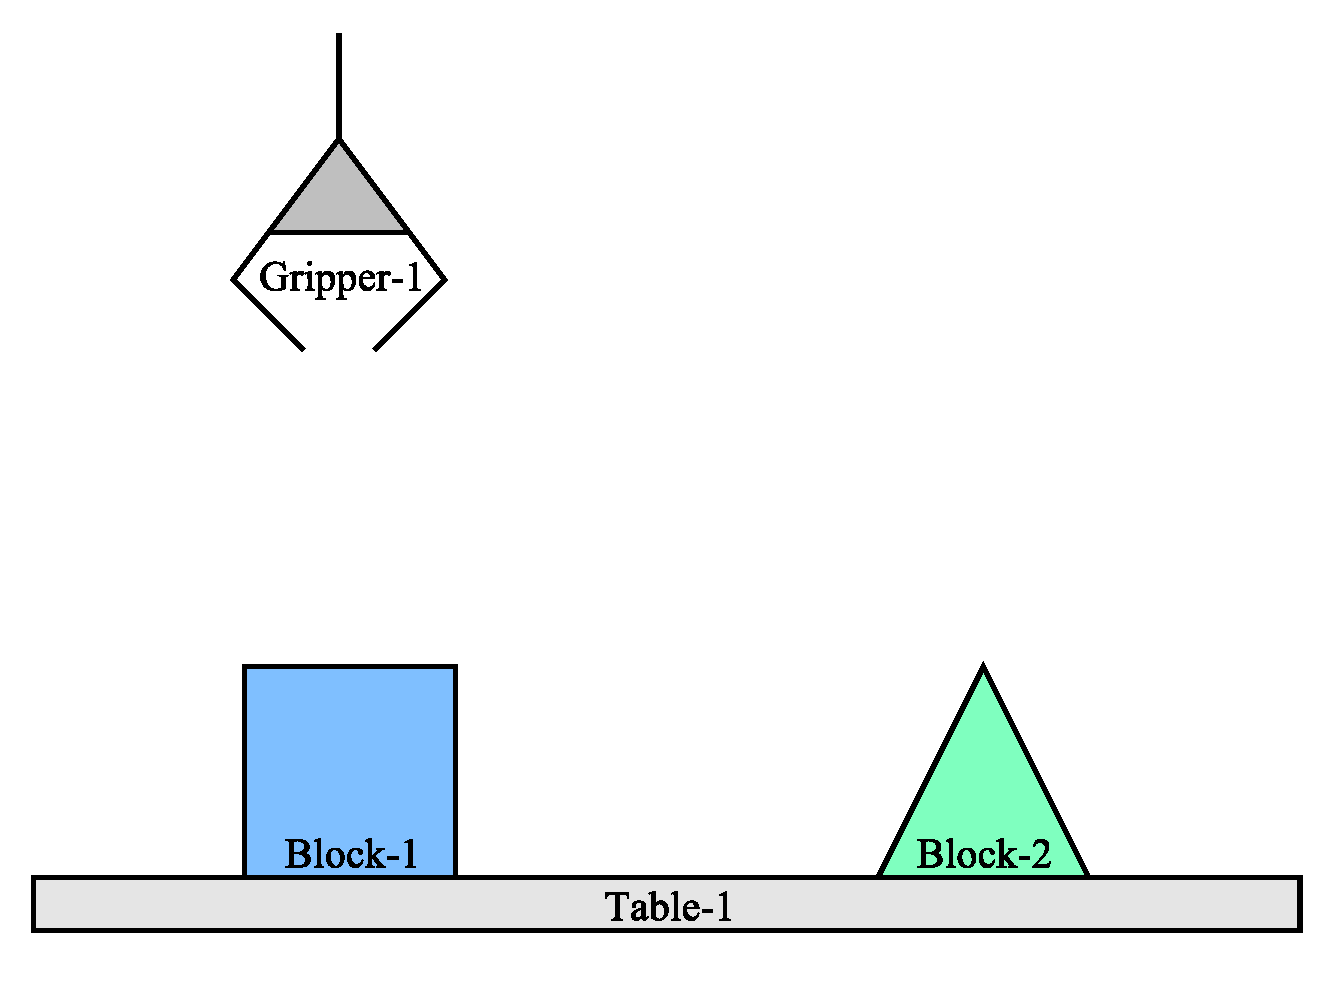
\includegraphics[width=4.5cm]{gfx/blocks_world_example-2} \\
3.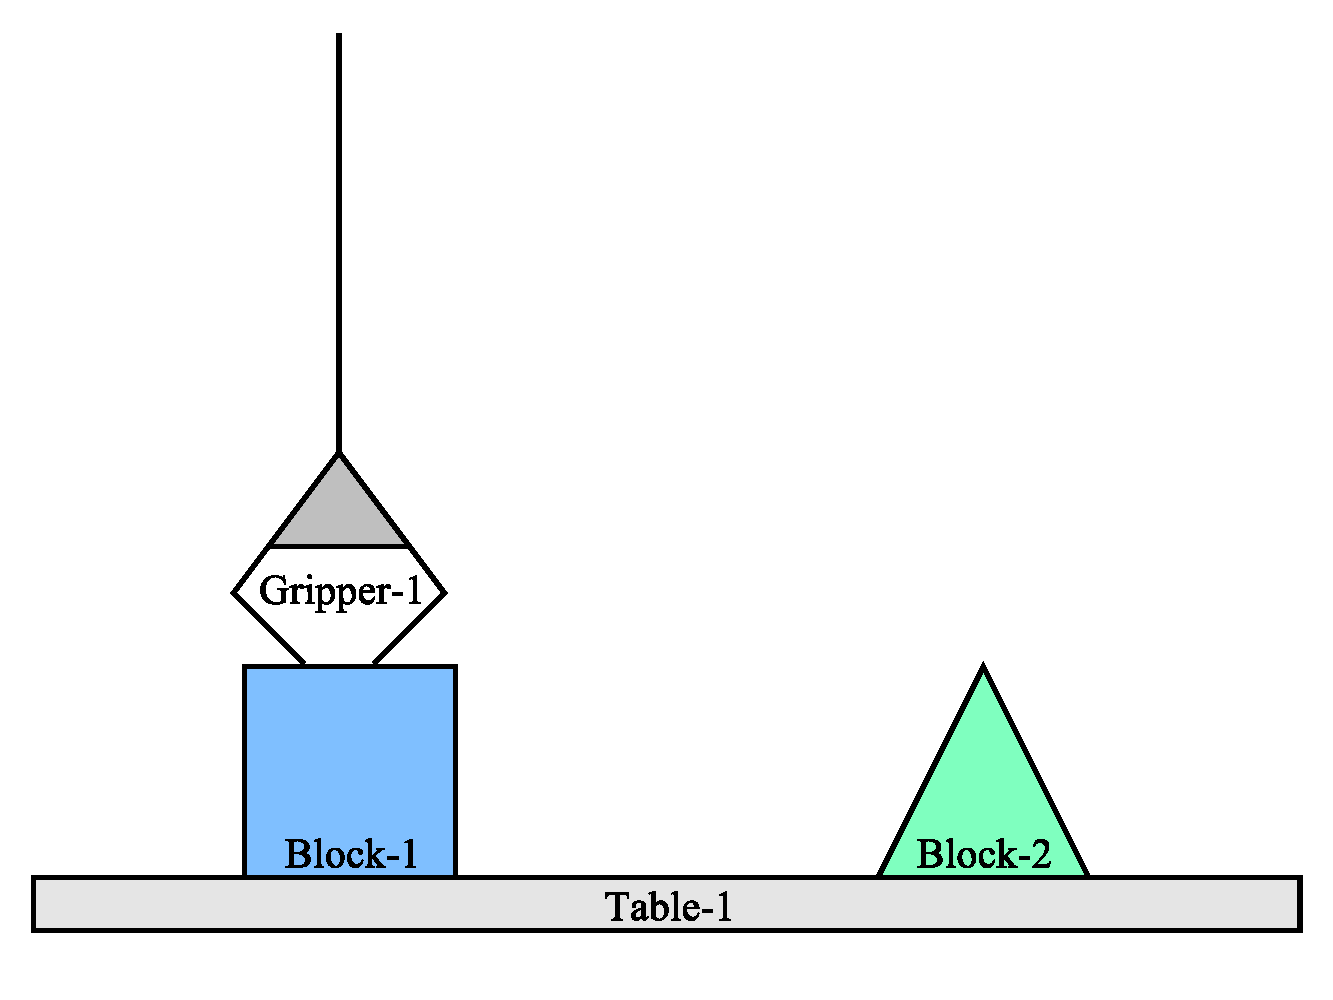
\includegraphics[width=4.5cm]{gfx/blocks_world_example-3} & 4.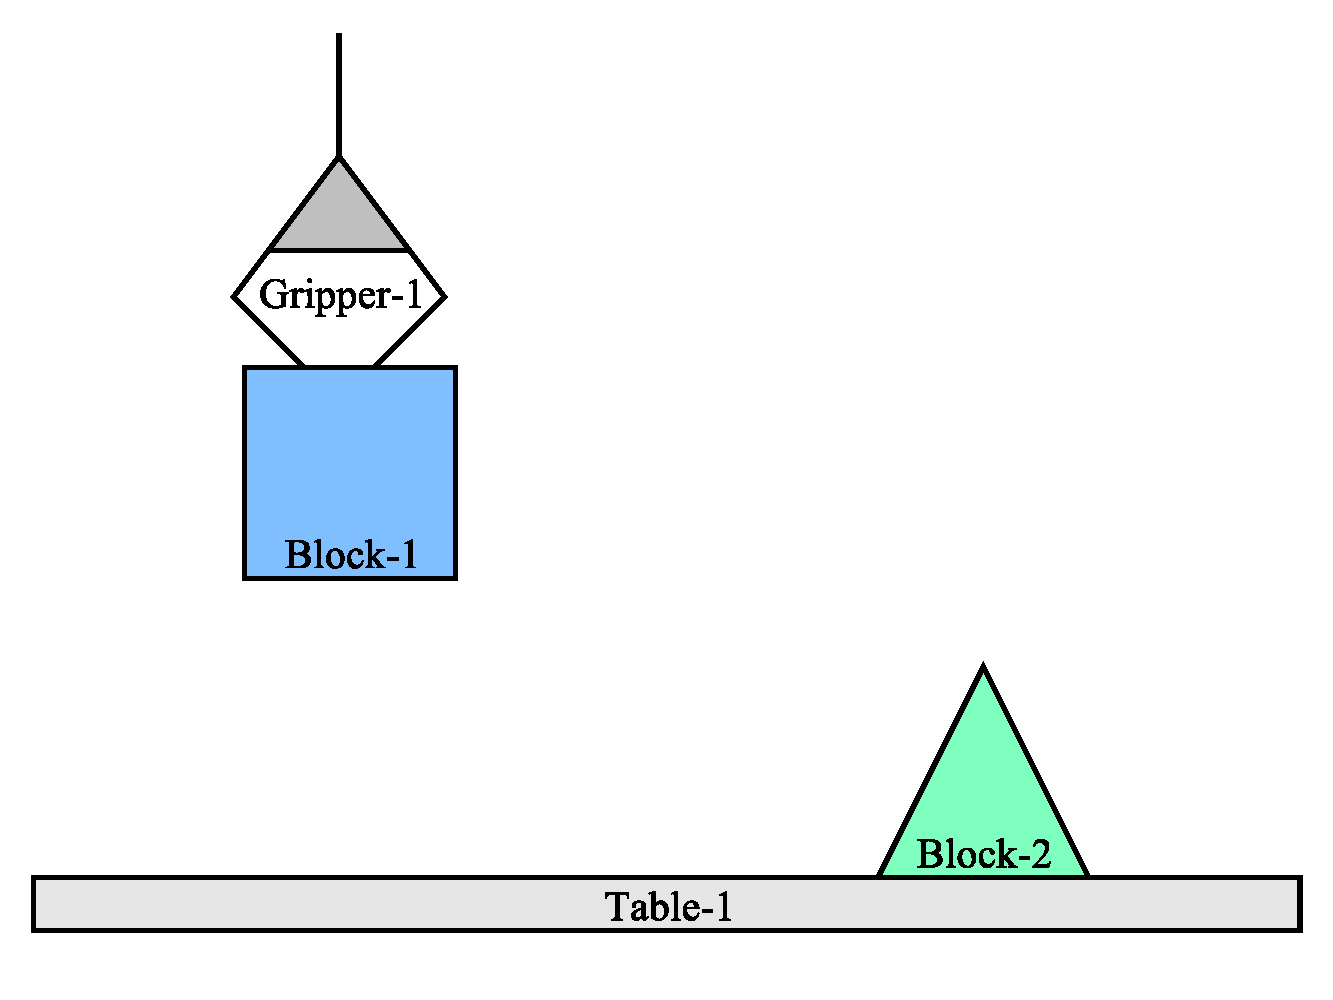
\includegraphics[width=4.5cm]{gfx/blocks_world_example-4} \\
5.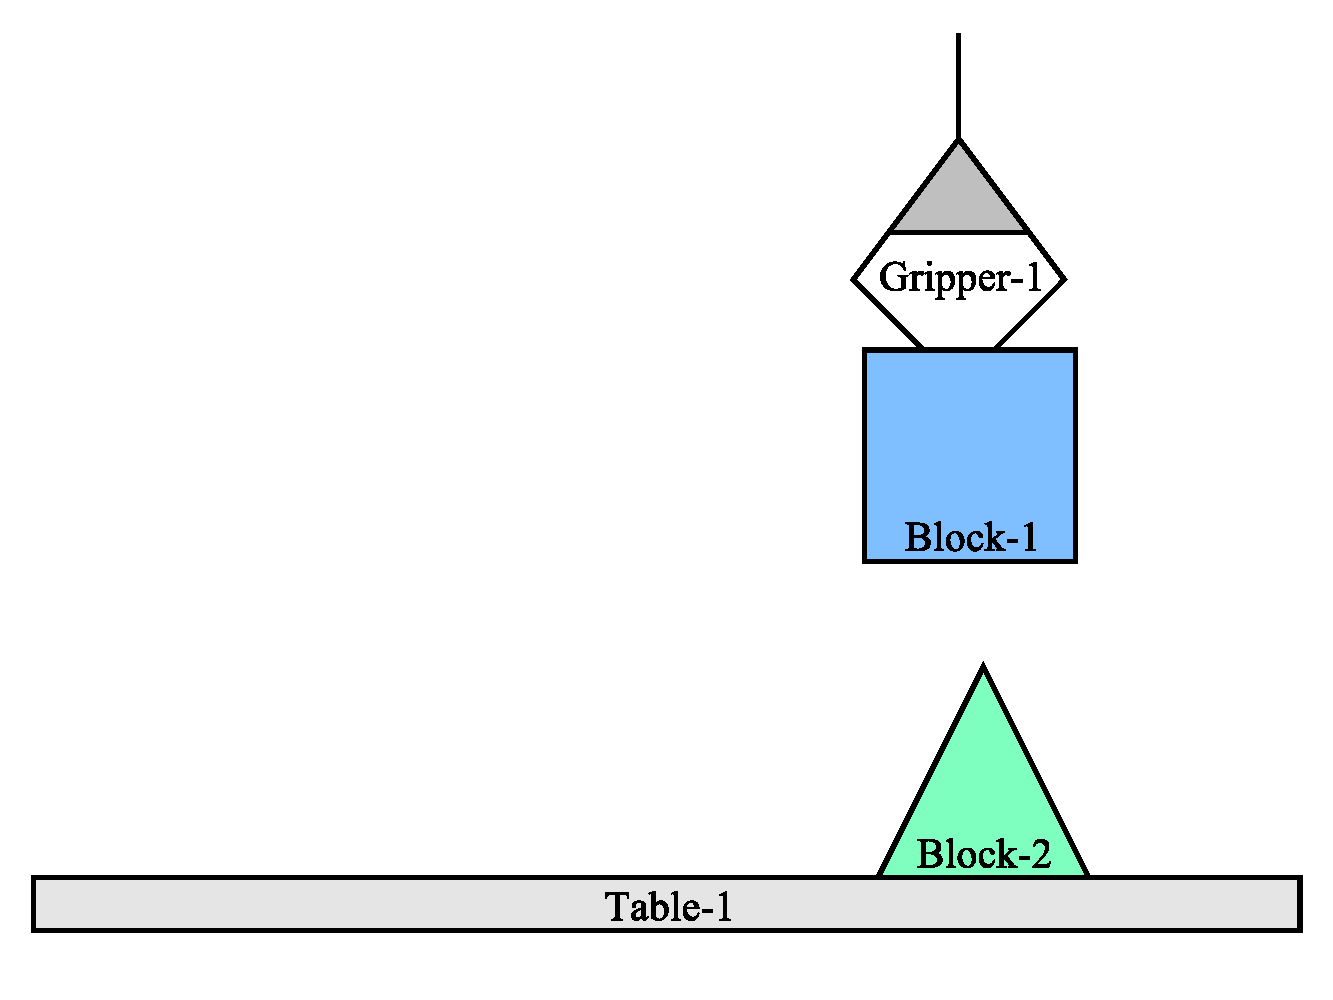
\includegraphics[width=4.5cm]{gfx/blocks_world_example-5} & 6.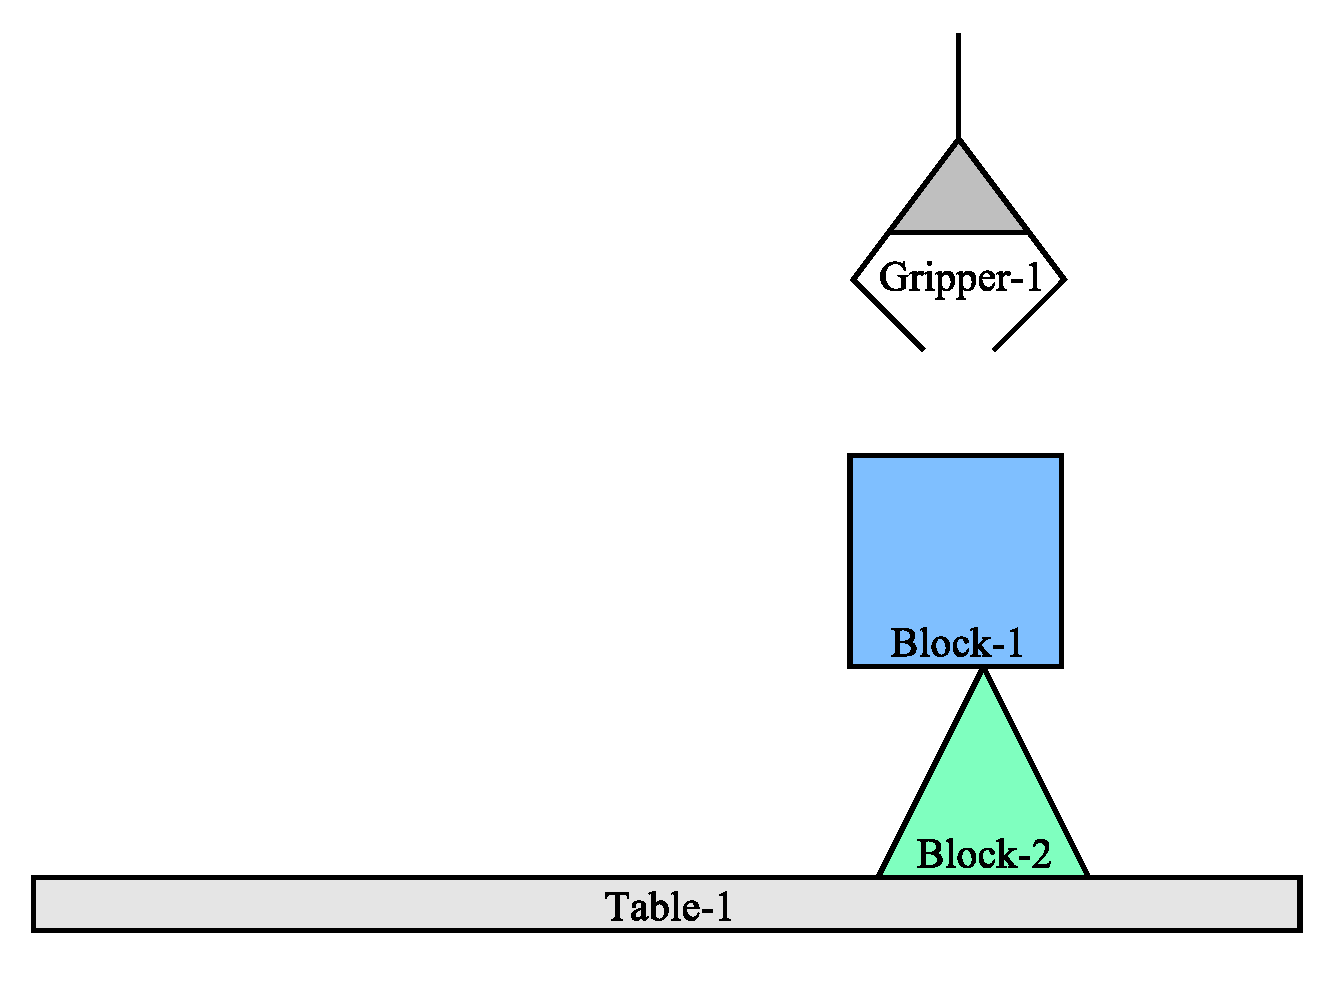
\includegraphics[width=4.5cm]{gfx/blocks_world_example-7}
\end{tabular}
\caption{An example of failure.}
\label{figure:blocks_world_example_of_failure}
\end{figure}

This is a common type of situation for current learning algorithms,
updating models of the world when experiences fail to match
expectations.  What I show in this thesis is that better models of
planning strategies can also be learned from these same failures.
Learning different planning strategies for different situations is a
reflective form of thinking.  Thus, my thesis is SALS, which provides
a working example of turning a single failure into failures at
multiple reflective layers, demonstrating multiple learning
opportunities from a single failure.

\section{Motivation}

\section{Explanation of the Problem}

\section{Contributions}

\section{Document Overview}

I begin with a non-technical description of the model in plain
English.  At the end of \autoref{part:the_model}, I explain the
modelling assumptions that I make in transitioning to the mathematical
notation of \autoref{part:simulating_the_model}.  Using this notation,
I explain how this model can be used to reduce the complexity of
search algorithms.  In \autoref{part:the_implementation}, I give an
explanation of how this simulation is automated on a concurrent
computer, the thesis implementation, SALS, the substrate for
accountable layered systems.  In conclusion, in
\autoref{part:conclusion}, I discuss promising directions for future
research in not only AI but also the other cognitive sciences.






